
%%% Local Variables:
%%% mode: latex
%%% TeX-master: t
%%% End:

\chapter{概述}

\section{背景} 
深圳市交通仿真系统(二期)构建了“ 1+2+2”的体系, 包括一个可动态更
新的多元交通、土地利用大数据平台, 以及专题数据挖掘分析系统、交通与土地
利用一体化交通模型系统、综合交通信息分析查询系统和面向多用户模型应用系
统四个子系统。

\begin{figure}[!hbt]
  \centering
  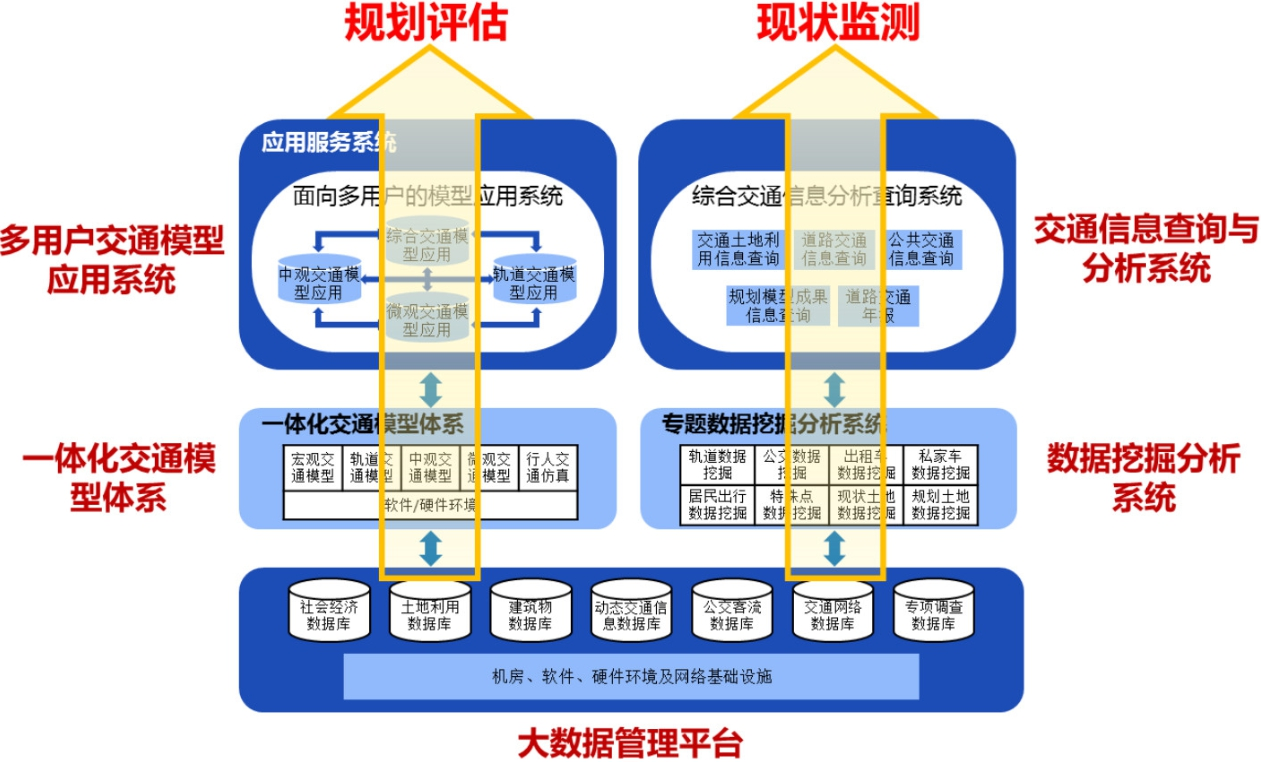
\includegraphics[width=\textwidth]{figures/项目体系架构.jpg}
  \caption{深圳市交通仿真系统(二期)的“ 1+2+2”体系\label{fig:项目体系架构}}
\end{figure}

其中, 深圳市交通仿真系统(二期) 项目已完成的工作包括:

\begin{para}
\item[多元数据平台] 负责对全市智能交通系统采集的动态交通数据、人口岗
位等社会经济数据以及土地利用、城市规划等 GIS 数据进行集中管理。
截止项目验收,数据更新至 2013 年 12 月;
\item[一体化交通模型体系] 全市宏观交通模型、罗湖区中观交通模型和大剧
院、大运会区域微观交通仿真模型和香蜜湖地铁站行人仿真模型;
\item[专题数据挖掘分析系统] 用于对多元数据平台的各类型数据按照交通和
土地利用指标进行挖掘分析,分析结果同样更新至 2013 年 12 月;
\item[面向多用户模型应用系统] 将一体化模型中的容积率、用地功能能重要
参数以接口形式提供出来, 由规划人员按照规划方案设定相关参数进行
模型运算,用以简化模型使用的难度;
\item[综合交通信息分析查询系统] 将专题数据挖掘分析系统中挖掘计算的各
类指标推送至浏览器前端,提供用户进行成果查询和展示的功能。
\end{para}

但是,在深圳市快速发展的背景下,为了能够更好地反映交通的特征和变化
趋势,以及构建快速响应的交通仿真模型,对深圳市交通仿真系统(二期) 原有
数据和已建成系统的更新工作具有十分重要的意义。

根据上述需求,项目组在原系统基础上,按照系统建设的规范和技术标准,每年度都会开展
基于上一年度数据和规划需求的模型和系统日常更新工作,并于\pyear 年10月完成了对
\ppyear 年数据的更新, 主要包括以下内容:

\begin{para}
\item[多元数据平台] 动态交通数据和静态 GIS 更新至\ppyear 年 12 月;
\item[数据挖掘和查询系统]各类指标分析结果至\ppyear 年;
\item[宏观轨道模型]现状年模型部分输入数据更新至\ppyear 年,且根据数据
挖掘成果更新和校核模型参数;
\item[中观交通模型]完善中观交通模型,新建龙华新区中观交通模型;
\item[微观交通模型]完成春风路隧道和梅林关车辆微观仿真模型建模工作。
\end{para}

因此,本项目作为年度常规更新项目,在原有系统的基础上, 主要目标是针
对 2015 年交通情况从底层数据平台到上层模型和信息化系统进行统一的更新。
一方面,通过系统的数据分析结果反映最新的现状交通特征, 并且可以通过与之
前年份的数据进行对比, 发现城市交通运行的变化趋势; 另一方面,通过更新工
作, 对原有模型系统进行补充和完善,提高原有模型精度,扩大模型建设范围,
为未来的交通规划工作提供定量依据和决策支撑。

\section{项目内容}
本项目延续了深圳市交通仿真系统(二期)“ 1+2+2” 的体系结构,更新的工
作主要包括数据更新、 信息化系统更新和模型更新三块内容。 其中,数据更新、
信息化系统更新在原有系统基础上, 按照深圳市交通仿真系统(二期) 系统设计
的更新技术要求进行常规类作业; 模型更新除在原有一体化模型体系基础上进行
常规性数据更新之外,还按照原有模型体系和建模技术要求, 新建福田区中观模
型和两个重点区域微观模型。 具体的工作可以分解为以下几个部分:

\smalltitle{数据更新}
在\pyear 年各类型动态交通数据和静态 GIS 数据基础上,采用人工编辑和自
动化处理相结合的技术方法对原始数据进行加工和处理,使其符合深圳市交通仿
真系统(二期) 中多元数据平台的入库要求,将原有系统中的数据扩充至 \pyear
年。

\smalltitle{数据挖掘系统更新}
在数据更新的基础上,采用自动化程序对\pyear 年各类交通指标数据进行重
新挖掘分析,在原有数据基础上扩充\pyear 年指标数据, 并将更新后的挖掘指标
推送至数据查询系统。

\smalltitle{宏观模型更新}
宏观模型更新的主要内容包括更新输入条件以及模型优化两方面。输入条件
更新包括综合网络更新、人口及土地利用数据、轨道OD矩阵更新等。模型优化的工作包括
收入模型、拥车模型和发生吸引模型。

\smalltitle{新建盐田、大鹏中观交通模型}
新建盐田区和大鹏新区中观交通模型,包括现状年模型和规划年模型。主要内容包括:
宏观模型截取区域路网及矩阵、小区及交通需求矩阵拆分、现场交通量调查、
模型校核、规划年路网更新、规划年需求矩阵预测、规划年新增用地交通需求叠加等工作。

\smalltitle{重点片区微观模型建设}
近年来,在城市轨道交通详细规划和交通枢纽改善规划等项目中,对交通枢纽建立行人微观仿真模型的
需求越来越多。因此,本项目基于行人仿真技术,新建大运枢纽规划行人仿真模型和高新园地铁站现状
行人仿真模型。

\smalltitle{数据查询系统更新}
在数据挖掘推送的指标数据基础上,采用自动化程序更新系统后台数据库,
并且在系统的前端将涉及到更新的功能展示出来, 使用户可以查询到 \pyear 年更
新的全部指标数据。

\smalltitle{数据查询系统更新}
在数据挖掘推送的指标数据基础上,采用自动化程序更新系统后台数据库,
并且在系统的前端将涉及到更新的功能展示出来, 使用户可以查询到 \pyear 年更
新的全部指标数据。

\smalltitle{系统运维}
针对深圳市交通仿真系统(二期) \pyear 年运行中出现的系统问题和异常进
行处理和维护, 并且在系统更新完成后进行年度的系统备份,保证系统的稳定运
行和异常恢复。

\section{技术路线}
\subsection{数据和信息化系统更新}
数据更新、数据挖掘系统更新和数据查询系统更新是承上启下的串行工作路
线,严格按照图中的流程进行作业, 但是每一部分内容内部又可以细分为并行流
程和串行流程; 相比前几项工作, 系统运维工作比较独立,备份工作需要在其他
所有工作完成后开展, 而其他两项工作可以在系统测试、 运行和使用的过程中同
步开展。

\begin{feai}
\item 城市更新\\
\indenttext{数据更新、数据挖掘系统更新和数据查询系统更新是承上启下的串行工作路
线,严格按照图中的流程进行作业, 但是每一部分内容内部又可以细分为并行流
程和串行流程; 相比前几项工作, 系统运维工作比较独立,备份工作需要在其他
所有工作完成后开展, 而其他两项工作可以在系统测试、 运行和使用的过程中同
步开展。}
\item 城市更新\\
\indenttext{数据更新、数据挖掘系统更新和数据查询系统更新是承上启下的串行工作路
线,严格按照图中的流程进行作业, 但是每一部分内容内部又可以细分为并行流
程和串行流程; 相比前几项工作, 系统运维工作比较独立,备份工作需要在其他
所有工作完成后开展, 而其他两项工作可以在系统测试、 运行和使用的过程中同
步开展。}
\item 我们\\
数据挖掘系统更新和数据查询系统更新是承上启下的串行工作路
线,严格按照图中的流程进行作业
\end{feai}

\begin{nbeae}
\item 数据更新\\
\indenttext{数据挖掘系统更新和数据查询系统更新是承上启下的串行工作路
线,严格按照图中的流程进行作业, 但是每一部分内容内部又可以细分为并行流
程和串行流程; 相比前几项工作,} 
\item 数据更新、数据挖掘系统更新和数据查询系统更新是承上启下的串行工作路
线,严格按照图中的流程进行作业, 但是每一部分内容内部又可以细分为并行流
程和串行流程; 相比前几项工作, 
\end{nbeae}

% \begin{para}
% \item[数据更新] 
% 数据挖掘系统更新和数据查询系统更新是承上启下的串行工作路
% 线,严格按照图中的流程进行作业, 但是每一部分内容内部又可以细分为并行流
% 程和串行流程; 相比前几项工作,
% \item[数据更新] 数据挖掘系统更新和数据查询系统更新是承上启下的串行工作路
% 线,严格按照图中的流程进行作业, 但是每一部分内容内部又可以细分为并行流
% 程和串行流程; 相比前几项工作, 
% \end{para}